\section*{Przegląd środowisk uruchomieniowych}
\addcontentsline{toc}{section}{Przegląd środowisk uruchomieniowych}
Do czasów powstania pierwszego środowiska uruchomieniowego JavaScript, możliwość uruchomienia programów ograniczał się do przeglądarki. Przeglądarki nie pozwalały na dostęp do pików, co nie pozwalało zapisywać dodatkowych plików na maszynie klienta. W ten sposób powstało pierwsze środowisko uruchomieniowe JavaScript w 2009, czyli NodeJS.

Środowiska uruchomieniowe pozwalają na uruchomienie skryptów JavaScriptu poza przeglądarką. Pozwoliło to językowi JavaScript stać się językiem generalnego użycia, co dla programistów stworzyło możliwość tworzenia aplikacji desktopowych, pozwoliło także na tworzenie API. Atutem powstałego w 2009 roku środowisko był asynchroniczny dostęp do systemu plików, pozwoliło to na optymalizacje operacji wejścia/wyjścia dla dużych skalowalnych aplikacji webowych.

Po upływie czasu zauważono, że NodeJS nie jest na tyle szybkim językiem do tworzenia serwerów, które mogły przekazywać informacje poprzez żądania HTTP. Stworzono także menadżera paczek, który pozwalał z jednego repozytorium pobierać paczkę, która umożliwiała uzupełnić braki samego środowiska. W czasie rosnącej popularności także zauważono, że rośnie liczba bibliotek, które korzystały z słabych punkty samego środowiska, dzięki którym pozyskano wrażliwe dane.

W odpowiedzi na narastające problemy związku działanie środowiska NodeJSm jego wolnym działaniem, zaczęto prace nad nowym bezpieczniejszym oraz wydajniejszym środowiskiem uruchomieniowym czyli Deno. Początkowo zostało zbudowane w oparciu o język Go, który został zamieniony na język Rust. Samo środowisko korzystało z silnika JavaScript stworzonego przez Google czyli V8. Twórcy Deno chcieli, aby paczki były dostępne pod linkiem, co oznacza szybsze przejście do samych pakietów. Dodatkowo Deno wprowadziło natywne wsparcie do TypeScript'a, pozwoliło to na statyczne typowanie samych bibliotek oraz zewnętrznych pakietów. Wersja 1.0 Deno, została wydana 13 maja 2020 roku.

Środowiska zostały wybrane na podstawie corocznej ankiety State of JS \cite{State_of_js:2022}, w której programiści wybierają narzędzia, które są przez nich najczęściej używane. Na liście z 2022 roku, można zauważyć, że nie został wymienione środowisko Bun,  spowodowane jest to wydanie wersji 1.0 we wrześniu 2023 roku. Możemy jednakże zauważyć, że Bun pojawia się w pracach \cite{NodeAndBun}, które analizują wydajność NodeJs oraz Bun.

Bun jako najmłodszy reprezentant środowisk wyróżnia się od pozostałych środowisk swoją szybkością, wbudowanym w sam silnik menadżer pakietów i bundler, co ułatwiło deweloperom kompresowanie samych aplikacji webowych. Środowisko to zostało napisane w języku Zig, dzięki czemu zawdzięcza swoją szybkość.

W tym rozdziale znajduje się opis wybranych do badań środowisk uruchomieniowych JavaScript.

\section*{NodeJS}
\addcontentsline{toc}{subsection}{NodeJS}
NodeJs jest to powstałe w 2009 środowisko uruchomieniowe, które pozwoliło na znaczne rozwinięcie samego środowiska języka JavaScript o dodatkowe funkcjonalności. Środowisko zostało oparte o silnik V8 od Google, które pozwoliło na uruchamianie kodu poza przeglądarką, które było do powstania środowiska niemożliwe. Wprowadziło to także możliwość tworzenia dynamicznych stron, co pozwoliło na rozwój bibliotek związanych z tworzeniem widoków. Aktualnie środowisko jest rozwijane przez OpenJs Fundation, sama organizacja wprowadza zmiany do samego środowiska np. obsługa zmiennych środowiskowych pobieranych z pliku.

Środowisko zostało zbudowane o paradygmat zdarzeniowy, stosuje się w nim pętle zdarzeniową, która nasłuchuje konkretnych zdarzeń, a następnie zdarzenia, które są umieszczone w stosie zdarzeń są wykonywane w kolejności FIFO. \cite{event_loop} Przedstawioną architekturę przedstawiono na Rysunku \ref{fig:eventLoop}.

\begin{figure}[h]
  \centering
  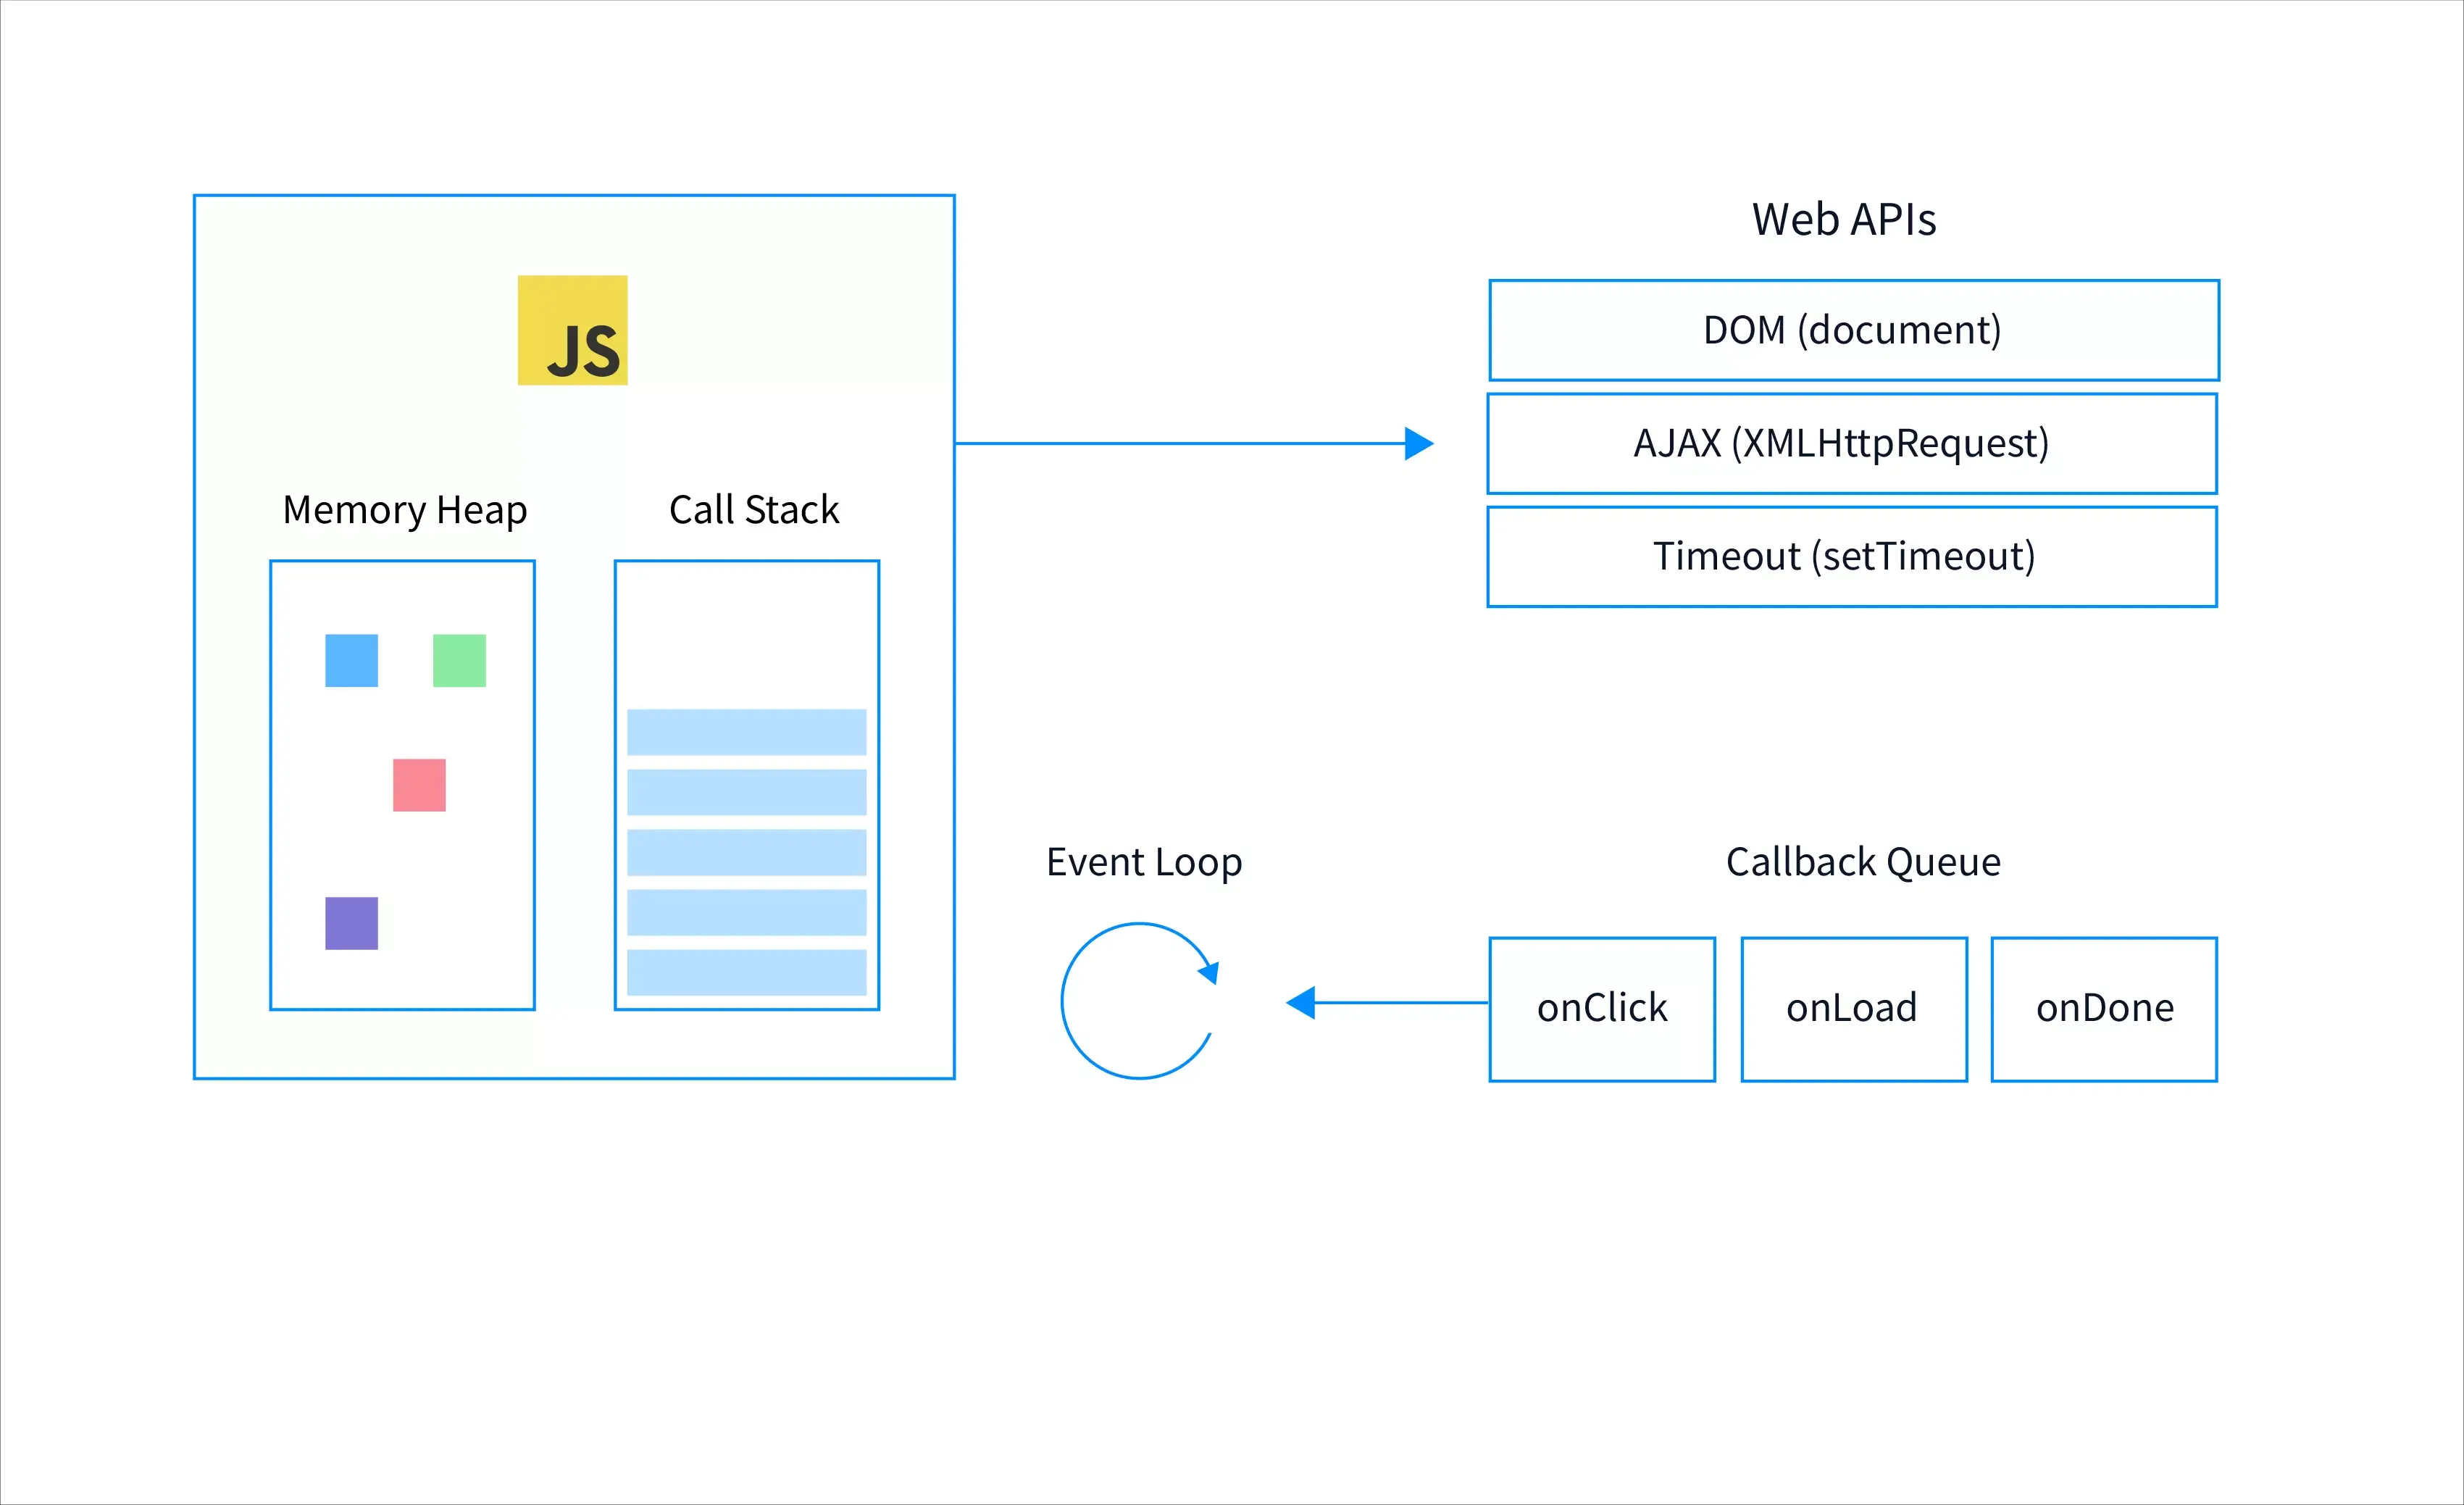
\includegraphics[width=0.9\textwidth]{Figures/eventLoop.png}
  \caption{Architektura zdarzeń}
  \label{fig:eventLoop}
\end{figure}

Zastosowanie powyższej architektury pozwoliło na wprowadzenie asynchronicznej obsługi operacji wyjścia wyjścia. Dzięki tej architekturze, NodeJs jest środowiskiem, w którym produkuje się skalowalne aplikacje internetowe. Środowisko to zostało rozwijane, gdzie dodatkowo wprowadzono moduły odpowiedzialne za funkcje kryptograficzne, funkcje odpowiedzialne za sieci oraz obsługę binarnych danych.

Środowisko posiada własny menadżer paczek, które są przeznaczone dla środowiska nazywający się npm. Npm został zaprezentowany w 2010 roku, rok od powstania samego środowiska. Korzystając z menadżer, deweloperzy mogą udostępniać biblioteki zrobione specjalnie pod NodeJs. Obecnie jest zarejestrowane 2.1 miliona bibliotek \cite{npm}, które znajdują się na w npm. Na przestrzeni czasu, można zauważyć, że Npm nie jest wydajnym menadżerem, dlatego też powstały alternatywy do npm takie jak: yarn oraz pnpm. 

W środowisku możemy pisać w kilku językach, niestety nie odbywa się to bez dodatkowej konfiguracji projektu. Sam NodeJs odczytuje tylko i wyłącznie programy transpilowane lub napisane w JavaScript. Na dzień dzisiejszy dzień środowisko wspiera transpilowanie w kilku języków takich jak: CoffeeScript, Dart, TypeScript oraz ClojureScript.

\section*{Deno}
\addcontentsline{toc}{subsection}{Deno}


\section*{Bun}
\addcontentsline{toc}{subsection}{Bun}
